\documentclass{article}
\usepackage{amsmath}
%\usepackage{subfigure}
\usepackage{subfig}
\usepackage{amsthm}
\usepackage{amssymb}
\usepackage{graphicx}
\usepackage{mdwlist}
\usepackage[colorlinks=true]{hyperref}
\usepackage{geometry}
\usepackage{titlesec}
\geometry{margin=1in}
\geometry{headheight=2in}
\geometry{top=2in}
\usepackage{palatino}
% \usepackage{mathrsfs}
\usepackage{fancyhdr}
\usepackage{paralist}
% \usepackage{todonotes}
\setlength{\marginparwidth}{2.15cm}
\usepackage{tikz}
\usetikzlibrary{positioning,shapes,backgrounds}
\usepackage{float} % Place figures where you ACTUALLY want it
\usepackage{comment}
\usepackage{ifthen}
\usepackage{biblatex}
\usepackage{courier}
\rhead{}
\lhead{}

\renewcommand{\baselinestretch}{1.15}

% Shortcuts for commonly used operators
\newcommand{\E}{\mathbb{E}}
\newcommand{\Var}{\operatorname{Var}}
\newcommand{\Cov}{\operatorname{Cov}}
\DeclareMathOperator{\argmin}{arg\,min}
\DeclareMathOperator{\argmax}{arg\,max}

% do not number subsection and below
\setcounter{secnumdepth}{1}

% custom format subsection
\titleformat*{\subsection}{\large\bfseries}

% set up the \question shortcut
\newcounter{question}[section]
\newenvironment{question}[1][]
  {\refstepcounter{question}\par\addvspace{1em}\textbf{Question~\Alph{question}\!
    \ifthenelse{\equal{#1}{}}{}{ [#1 points]}: }}
    {\par\vspace{\baselineskip}}

\newcounter{subquestion}[question]
\newenvironment{subquestion}[1][]
  {\refstepcounter{subquestion}\par\medskip\textbf{\roman{subquestion}.\!
    \ifthenelse{\equal{#1}{}}{}{ [#1 points]:}} }
  {\par\addvspace{\baselineskip}}

\titlespacing\section{0pt}{12pt plus 2pt minus 2pt}{0pt plus 2pt minus 2pt}
\titlespacing\subsection{0pt}{12pt plus 4pt minus 2pt}{0pt plus 2pt minus 2pt}
\titlespacing\subsubsection{0pt}{12pt plus 4pt minus 2pt}{0pt plus 2pt minus 2pt}



\chead{%
  {\vbox{%
      \vspace{2mm}
      \large
      Networks: Structure \& Economics \hfill
      Caltech CMS/CS/EE 144 \hfill \\[1pt]
      Miniproject 1\hfill
      February $8^{\text{rd}}$, 2016 \\
    }
  }
}

\begin{document}
\pagestyle{fancy}

\LARGE
\begin{center}
\textbf{Churn}

\large
John Li, Albert Ge, Timothy Chou, Kevin Chang

Rankmaniac Report

\end{center}

\normalsize
\medskip

\section{Overview}
During this Pandemaniac project, our group ``churn'' implemented a number of algorithms to choose 
seed nodes in a network to optimize the spread of a simulated epidemic across the graph. 
The code was written in a Python base. 

\subsection*{Counterexample}
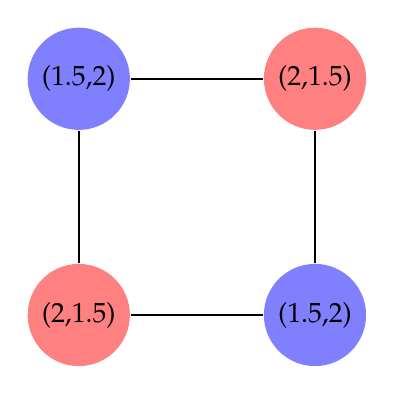
\begin{tikzpicture}[auto,node distance=3cm, thick,main node/.style={circle,fill=blue!50,minimum size=1cm},sub node/.style={circle,fill=red!50,minimum size=1cm}]
\node[main node] (1) {(1.5,2)};
\node[sub node] (2) [right of=1] {(2,1.5)};
\node[sub node] (3) [below of=1] {(2,1.5)};
\node[main node] (4) [right of=3] {(1.5,2)};

\path[draw, thick]
(1) edge node {} (2)
edge node {} (3)
(4) edge node {} (2)
edge node {} (3)
;
\end{tikzpicture}\\
Next iteration is\\
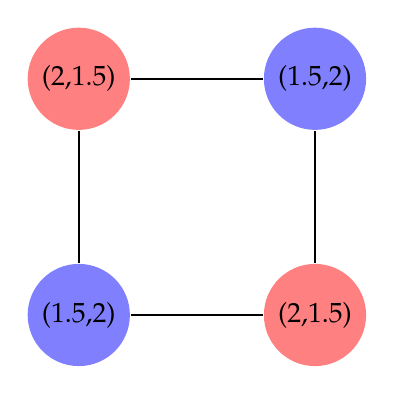
\begin{tikzpicture}[auto,node distance=3cm, thick,main node/.style={circle,fill=blue!50,minimum size=1cm},sub node/.style={circle,fill=red!50,minimum size=1cm}]
\node[sub node] (1) {(2,1.5)};
\node[main node] (2) [right of=1] {(1.5,2)};
\node[main node] (3) [below of=1] {(1.5,2)};
\node[sub node] (4) [right of=3] {(2,1.5)};

\path[draw, thick]
(1) edge node {} (2)
edge node {} (3)
(4) edge node {} (2)
edge node {} (3)
;
\end{tikzpicture}\\
Which we see cycles back to \\
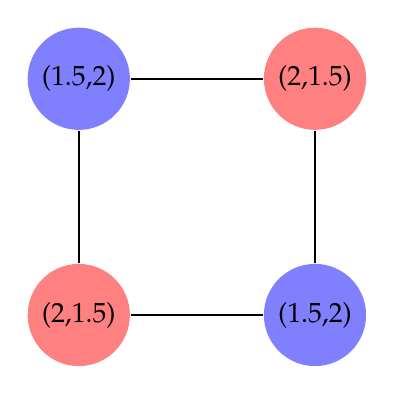
\begin{tikzpicture}[auto,node distance=3cm, thick,main node/.style={circle,fill=blue!50,minimum size=1cm},sub node/.style={circle,fill=red!50,minimum size=1cm}]
\node[main node] (1) {(1.5,2)};
\node[sub node] (2) [right of=1] {(2,1.5)};
\node[sub node] (3) [below of=1] {(2,1.5)};
\node[main node] (4) [right of=3] {(1.5,2)};

\path[draw, thick]
(1) edge node {} (2)
edge node {} (3)
(4) edge node {} (2)
edge node {} (3)
;
\end{tikzpicture}\\
Meaning equilibrium will never be reached. 
\section{Initial Framework}
    We began this project by first understanding and processing the data from the format of a JSON file.
    We wrote some initial files to load the data from a JSON file, and use some naive algorithm to
    pick seed nodes (described below).
    To present it in a file suitable for submission, a file \texttt{submit.py} was 
    created, which took in as its parameter the graph input file, and output results in a file
    \texttt{submit.txt} for upload.
    
    \subsection*{Early Bird Points} 
    To obtain early bird points, we first wrote a short file \texttt{deg\_centrality.py} which
    ranks the top X nodes by their degree value. Here X refers to the number of seeds
    to be picked, as denoted by the name of each graph JSON file. 
    
    \subsection*{Beating TA\_fewer and TA\_degree}
    The next algorithm we tried was tailored specifically to beat TA\_degree
    written in \texttt{deg\_centrality2.py}. Given that
    TA\_degree follows the exact same strategy, then all of the initial seed pickings
    would be cancelled by TA\_degree. To combat this, we would pick the top X-1 seeds by degree,
    and the last seed to just be a neighbor of the highest-degree node. The intuition 
    behind this is that, as the top X-1 nodes would be cancelled out, TA\_degree would be 
    left with the Xth-highest degree node, and we would have a neighbor to the 
    highest degree node. Thus, after a single step in a round, we would (ideally) obtain
    control of the highest degree node. 
    \\
    This algorithm ended up beating both TA\_fewer and TA\_degree, securing the remaining
    required points for the programming side of the project. 
     

\section{Development and Improvements}

\subsection*{Top-K Mix}
This algorithm involved finding the degree centrality. closeness centrality, and betweeness centrality, then selecting the top $A, B, C$ respectively from each. 

\subsection*{Linear Combinations}
The idea was that nodes with high measures of centrality, specifically degree centrality, closeness centrality, and betweenness centrality, would be the best nodes to choose in a 2-player game. This model ignores remote clusters because we assume that since there are only two players and we have so few seed nodes, we need to contest the central area. What is unclear is which measure of centrality is most important, so we assumed the best model would be a linear combination of these three centrality measures. 
${Score}(x) = \alpha * {Betweenness-Centrality}(x) / 0.07 + \beta * {Closeness-Centrality}(x) / 0.54 + \gamma * {Degree-Centrality}(x) / 0.28$
We found maximum Betweenness Centrality, Closeness Centrality, and Degree Centrality of the versus-TA graphs to be approximately 0.07, 0.54, 0.28 respectively. Thus we hard coded these to normalize the contributions due to the three centrality measures.

\subsection*{PageRank}
Looking at the graphs, we realized that if a node is near central nodes, it also gains some importance. We therefore implemented a 1-step PageRank-like algorithm that simply increases the score of each node by the score of each neighbor divided by degree of that neighbor. However, this did not seem to improve performance, so we did not use this in our actual runs.

\subsection*{Monte Carlo}
Monte Carlo simulations were done on the various linear combinations and top-K mixes. A number of samples of different linear combinations incrementing $\alpha$, $\beta$, and $\gamma$ in .05 steps forcing $\alpha + \beta + \gamma = 1$ and every possible selection of A, B, C for a top-K mix was used to represent different strategies we were considering generating different seeds on 16 graphs. In addition, we also hand selected seeds in an attempt to immitate TA\_more. We then pitted all the strategies against each other, with one side getting the normal amount of seeds and the player 2 getting 20\% more seeds. Doing so involved playing approximately 2 million games, so the simulation was run (\texttt{runSim.py}) across multiple computers before the outputs were agreggated using \texttt{combineResults.py}. These results were then used for our final attempt against TA\_more. The final result was a linear combination with weights $[.70, .25, .5]$ which had won at least 5 out of 16 graphs against every player 2 (which had 20\% more seed nodes). 

\subsection*{Bridges}
  In the structure of the graph, we noticed that access to strongly connected components is 
  very important if we want to spread our influence throughout the graph. However, the only way to move from one strongly connected component to the other is through bridge edges. Since an edge only attaches one vertex with another, entrance to another connected component must first begin by going through the gateway node at the other end of the bridge edge. I will refer to these nodes as ``bridge nodes'' from here on out. 
  \\ \\
  Because of this, we noticed that taking control over some of these bridge nodes would be very valuable, as they secure a place in one of the connected components, it can prevent other players from entering a component, and it gives easier access to an adjacenct connected component. Therefore, this optimization relied on finding bridge nodes, ranking the bridge nodes based on a significance measure (more on that later), and then including these bridge nodes in the final submission.
  \\ \\
  Now, we first need to find these bridge nodes. The naive approach would be to remove each node, and then call a searching algorithm to determine whether or not the search would return the same number of visited nodes. However, this would require us to call the searching algorithm a total of $V$ times, where $V$ represents the number of vertices. So, this would be polynomial time, and while it is still poly-time, the size of the graph may be so large that we would not produce results within the time constraints. So, what we did instead was to use a linear-time bridge-finding algorithm. In particular, we used Tarjan's Bridge Finding Algorithm$^1$. The algorithmic steps are below, followed by brief implementation details that we did:
  
  \begin{verbatim}
  Tarjan's Algorithm:
    1: Find a spanning forest of graph G
        - This was done using DFS until the entire graph is searched.

          If the DFS finishes without the entire graph searched, start 
          another DFS on an unvisited node, since it should be on a 
          new connected component.

        - Return value: Adjacency Matrix/Matrices of the directed spanning 
          forest.

    2: In the spanning tree, order all the nodes in preorder (order which you
       discovered them in your DFS)

        - A map was created mapping each node to its respective preorder.
          This proved very useful for later dynamic programming things.

    3: Going in reverse preorder order, we calculate each nodes respective
       lower bound, higher bound, and the number of descendants it has.

       - All three were done in reverse preorder order, so that we could
         use dynamic programming. Dynamic programming table was an array
         with each index of the array representing the preorder value of 
         a node 'n'. This is why the map comes in handy.

       - ND(n), for node n, is calculated by adding the number of descendants
         held by n's children. We then add 1 to include 'n' itself into the
         count.

       - L(n) and H(n) were calculated by first examining all edges not in
         the tree, and finding the minimum/maximum preorder value of its
         neighbors. Then, we compare that with the L/H values of 
         its children in the spanning tree. We take the minimum/maximum of
         that for L(n)/H(n) values.

    4: Going in preorder order, we check each spanning tree edge (u -> v),
       and if:
       1) L(v) = PreOrder(v) AND
       2) H(v) < PreOrder(v) + ND(n)

       then (u, v) is a bridge edge and u, v are bridge nodes.
  \end{verbatim}

  Once we find the bridge edges, that's just the first part. We now have to choose which bridge edges are valuable in the graph, and which ones are not worth choosing. For example, many bridge edges actually end up being edges that connect to an endpoint in the graph (a vertex with a degree of just 1).
  It is obvious that these bridge nodes are not worth adding, since they do
  not really capture the strongly connected components we were looking for.
  \\ \\
  Therefore, after finding the bridge nodes, one thing we did was to rank the value of bridge nodes through the following ways:
  \begin{enumerate}
    \item We would rank the bridge nodes solely by degree
    \item We would rank the bridge nodes both by degree and the size of its
          connected component compared with the size of the rest of the
          graph.
  \end{enumerate}

  Through trial and error and by using multiple json graphs, we ended up using
  the following format:
  \begin{verbatim}
    |V|/2 = halfGraph
    Ranking each bridge node:
      Find the size of its connected component (sizeOfComponent)
      Find the size of the rest of the graph (remainingPart)
      Find its degree (degree)
      Rank the bridge node with the following expression:
        Rank = (sizeOfComponent * (remainingPart + degree) / 
                halfGraph^2 - sizeOfComponent * remainingPart + 1)
  \end{verbatim}

  We sorted these rankings where larger ranks equate to more value. While the 
  full ranking hasn't been completely developed, this ranking system is explained below: \\ \\
  \textsc{Numerator}: \\
  We want to maximize this numerator. We want large degrees since this means
  that this bridge node is not just connected to another component, but also to many vertices in its own component. Further, we wanted the size of the 
  partition to matter as well: we want control of larger partitions rather
  than small ones. Though both are important, it is more important to
  secure a spot in a larger component.
  \\ \\
  \textsc{Denominator}: \\
  We want to minimize this number, for larger rankings. First, we don't want
  the size of the partition sizes to be that different. This is to account for nodes involved in ``endpoints'' or in really really small connected 
  components, which just really aren't that valuable. Even with a larger
  neighbor partition, it is not worth a node to block its entrance from a
  smaller connected component. The random ``$+ 1$'' is added to ensure
  that we don't divide by 0 (say, if a bridge node actually has a partition
  size of half the graph)
  \\ \\
  Another problem with this system, however, is that this ranking system
  will take a very long time for large graphs, since finding partition sizes 
  involves searching through each bridge node. Once again, this is, at worst,
  polynomial time, which can cause a lot of time for large graphs. So, we
  add one more constraint, where if the number of vertices is greater than 
  1000, we limit the depth of the search to be only $K$ vertices deep, where $K$ is an integer that we tweak. This transforms the time from polynomial to linear. Although accuracy takes a hit, it allows us to provide ranks for
  larger graphs on time.
  \\ \\
  Finally, once the bridge nodes are found and ranked, we output all the 
  bridges in a text file \texttt{bridgeNodes.txt}. This is then used for
  the mixed strategy illustrated below: we do not want to solely pick 
  bridge nodes because we can never be sure that a graph has bridge nodes.
\subsection*{Mixed Strategy}
    Using a mixed strategy requires some notion picking seed nodes according to some
    probability distribution. Each strategy will output 
    the rankings of the top X nodes, according to some centrality measure, 
    which provides a quantitative notion of how important a particular seed is relative 
    to others. Thus, our idea was to use the values of centrality measure as a rough
    probability of how likely it is to be selected as a node - the greater the measure,
    the more likely it is to be picked. This follows similarly with the idea of computing
    the probabilities of a mixed strategy - a particular action receives greater 
    probability if its expected payoff is greater. 
    \\
    In a file, \texttt{mixed.py}, we outline the procedure for computing a mixed strategy.
    Assuming that all centrality measures are equally important, we pick one of the
    measures at random, obtain a list of most important nodes according to that measure,
    and perform a weighted random choice among those nodes.
    \\
    \textbf{Results:} Using a mixed strategy for the bridge centrality measure,
    and degree centrality, we obtained a score of 2 on day3 of 
    the tournament. Though it wasn't much,
    this was the most points we've scored out of all three days of the tournament,
    and it seemed to be a promising avenue to explore given more time.
    
\section{Testing}
    We tested the algorithms for computing seed nodes by running them against
    each other, using the provided \texttt{sim.py}. To facilitate this,
    a wrapper class \texttt{runStrat.py} was created, which takes as arguments
    a variable number of strategies and a graph input, picks the seeds according to each strategy,
    and runs the simulation with seeds on the graph.



 % Can talk about data mining. What scripts we used. etc.
 

\section{Contributions}
There are four members in this group: Kevin Chang, Timothy Chou, Albert Ge, and John Li. Here are each of their contributions:
\begin{itemize}
  \item \textsc{Kevin Chang}: Wrote linear combination strategy generator \texttt{create\_strats.py}
  \item \textsc{Timothy Chou}: Wrote and designed algorithm to beat TA\_degree. Wrote monte carlo simulator \texttt{runSim.py}, wrote mixed top-K strategy in \texttt{create\_strats.py} and ran tests to find optimal linear combination.
    \item \textsc{Albert Ge}: Wrote most of the initial framework - \texttt{deg\_centrality.py}, \texttt{submit.py}, 
  Wrote the testing script \texttt{runStrat.py}. 
  Wrote \texttt{mixed.py}, the script for employing mixed strategies according to
  a probabilistic distribution.
  \item \textsc{John Li}: Studied Tarjan's linear-time bridge detection algorithm and wrote all of \texttt{bridges.py}. Also developed \texttt{pagerank.py} before migrating it into another file. 
 % Should be on FB chat.
 \end{itemize}

\section{Citations}
\begin{enumerate}
  \item Tarjan's Bridge Finding Algorithm: \\
  https://en.wikipedia.org/wiki/Bridge\_(graph\_theory)\#Tarjan.27s\_Bridge-finding\_algorithm
\end{enumerate}

%\section{Model Selection}
%Describe the steps you took to pick your final model, such as cross-validation.

%\section{Conclusion}
%Conclude with the overall performance of your project. Mention any possible improvements.


\end{document}
